% This file demonstrates how to use the IEEEConf LaTeX2e macro package,
% to prepare a manuscript for proceedings on CD of the conference
% FedCSIS
%
\documentclass[conference]{IEEEtran}
%\documentclass[a4paper]{IEEEconf}

% This package serves to balance the column lengths on the last page of the document.
% please, insert \balance command in the left column of the last page
\usepackage{balance}

%% to enable \thank command
\IEEEoverridecommandlockouts 
%% The usage of the following packages is recommended
%% to insert graphics
\usepackage{graphicx}
% to typeset algorithms
%\usepackage{algorithmic}
\usepackage{algorithm}
% to typeset code fragments
\usepackage{listings}
% to make an accent \k be available
\usepackage[OT4,T1]{fontenc}
% provides various features to facilitate writing math formulas and to improve the typographical quality of their output.
\usepackage[cmex10]{amsmath}
\interdisplaylinepenalty=2500
% por urls typesetting and breaking
\usepackage{url}
% for vertical merging table cells
\usepackage{multirow}

\usepackage{filecontents}

\usepackage{color}
\usepackage{xcolor}
\usepackage{colortbl}
\definecolor{LightCyan}{rgb}{0.88,1,1}
\definecolor{BluishGray}{RGB}{226,227,231}
\definecolor{LightGray}{gray}{0.95}
\definecolor{Gray}{gray}{0.85}
\usepackage{algpseudocode,algorithmicx}
\usepackage{comment}
\newcommand*\DNA{\textsc{dna}}

\newcommand*\Let[2]{\State #1 $\gets$ #2}
\algrenewcommand\algorithmicrequire{\textbf{Input:}}
\algrenewcommand\algorithmicensure{\textbf{Output:}}
\algrenewcommand\algorithmicrequire{\textbf{Input:}}
\algrenewcommand\algorithmicensure{\textbf{Output:}}

% define environments for remarks and examples
\newtheorem{remark}{Remark}[section]
\newtheorem{example}[remark]{Example}
\newcommand{\ti}{\textit}
\newcommand{\tb}{\textbf}




%
%
\title{???!}
%
%
\author{
\IEEEauthorblockN{Van Cam Pham, Ansgar Radermacher, Sebastien Gerard}
\IEEEauthorblockA{
CEA-List, Laboratory of Model-Driven Engineering for Embedded Systems (LISE)\\
Gif-sur-Yvette, France\\
Email: first-name.lastname@cea.fr}
}

% conference papers do not typically use \thanks and this command
% is locked out in conference mode. If really needed, such as for
% the acknowledgment of grants, issue a \IEEEoverridecommandlockouts
% after \documentclass

% for over three affiliations, or if they all won't fit within the width
% of the page, use this alternative format:
% 
%\author{\IEEEauthorblockN{Michael Shell\IEEEauthorrefmark{1},
%Homer Simpson\IEEEauthorrefmark{2},
%James Kirk\IEEEauthorrefmark{3}, 
%Montgomery Scott\IEEEauthorrefmark{3} and
%Eldon Tyrell\IEEEauthorrefmark{4}}
%\IEEEauthorblockA{\IEEEauthorrefmark{1}School of Electrical and Computer Engineering\\
%Georgia Institute of Technology,
%Atlanta, Georgia 30332--0250\\ Email: see http://www.michaelshell.org/contact.html}
%\IEEEauthorblockA{\IEEEauthorrefmark{2}Twentieth Century Fox, Springfield, USA\\
%Email: homer@thesimpsons.com}
%\IEEEauthorblockA{\IEEEauthorrefmark{3}Starfleet Academy, San Francisco, California 96678-2391\\
%Telephone: (800) 555--1212, Fax: (888) 555--1212}
%\IEEEauthorblockA{\IEEEauthorrefmark{4}Tyrell Inc., 123 Replicant Street, Los Angeles, California 90210--4321}}





\begin{document}
\maketitle              % typeset the title of the contribution

\begin{abstract}
%The so-called model-driven engineering approach relies on two paradigms, abstraction and automation, recognized as very efficient for dealing with complexity of today system. 
%Abstraction is the ability to provide simplified and focused view of a system and requires adequate modeling language. 
%For this concern, it is clear that the Unified Modeling Language (UML) is nowadays the most used, educated, documented and tooled modeling language. 
%Even, if a graphical language such as the UML is not the silver bullet for all software related concerns, it provides hence better support than text-based solutions for some concerns such as architecture and logical behavior of application development. 
UML state machine and their visual representations are much more suitable to describe logical behaviors of system entities than any equivalent text based description such as IF-THEN-ELSE or SWITH-CASE constructions. Although many industrial tools and research prototypes can generate executable code from such graphical language, generated code could be manually modified by programmers. 
After code modifications, round-trip engineering is needed to make the model and code consistent, which is a critical aspect to meet quality and performance constraint required from project manager today. Unfortunately, current UML tools only support structural concepts for round-trip engineering such as those available from class diagrams. In this paper, we address the round-trip engineering of UML state-machine and its related generated code. We propose a round-trip engineering approach consisting of a forward process which generates code by using transformation patterns, and a backward process which is based on code pattern detection to update the original state machine model from the modified generated code. We implemented a prototype and conducted several experiments on different aspects of the round-trip engineering to verify the proposed approach.


%Unified Modeling Language (UML) State machine is widely used 

%Model-driven engineering (MDE) is a development methodology aiming to increase software productivity and quality by automatically generating code from higher level abstraction models. 
%A recent survey has revealed that industries are gaining the adoption of code generation into software development life-cycle. 
%Although many tools and research prototypes can generate executable code from models (e.g. Unified Modeling Language), developers, after code generation, tend to abandon models and code generators in software evolution. The reason behind is that generated code could be manually modified by developers and code modifications are not easily propagated back to models. Round-trip engineering (RTRIP) supported by many tools is needed to make the model and code consistent but most of the tools are only applicable to static diagrams such as classes. In this paper, we tackle a classical problem : from UML State Machine diagrams to code and back. We propose a RTRIP approach consisting of a forward process, which generates code, and a backward process, which updates the original state machine from the modified generated code. From the proposed approach, we implemented a prototype and conducted several experiments on different aspects of the round-trip engineering to verify the proposed approach.
\end{abstract}

\begin{comment}
\section{Figures and Tables}
To insert a figure you are encouraged to use the  \verb|graphicx| package. Please, include this package in the preamble with the option \verb|dvips|:
\begin{verbatim}
\usepackage[dvips]{graphicx}
\end{verbatim}
Figures in the \verb|eps| format should be inserted in the \verb|figure| environment, as follows:
\begin{verbatim}
\begin{figure}[tbp]
\centering
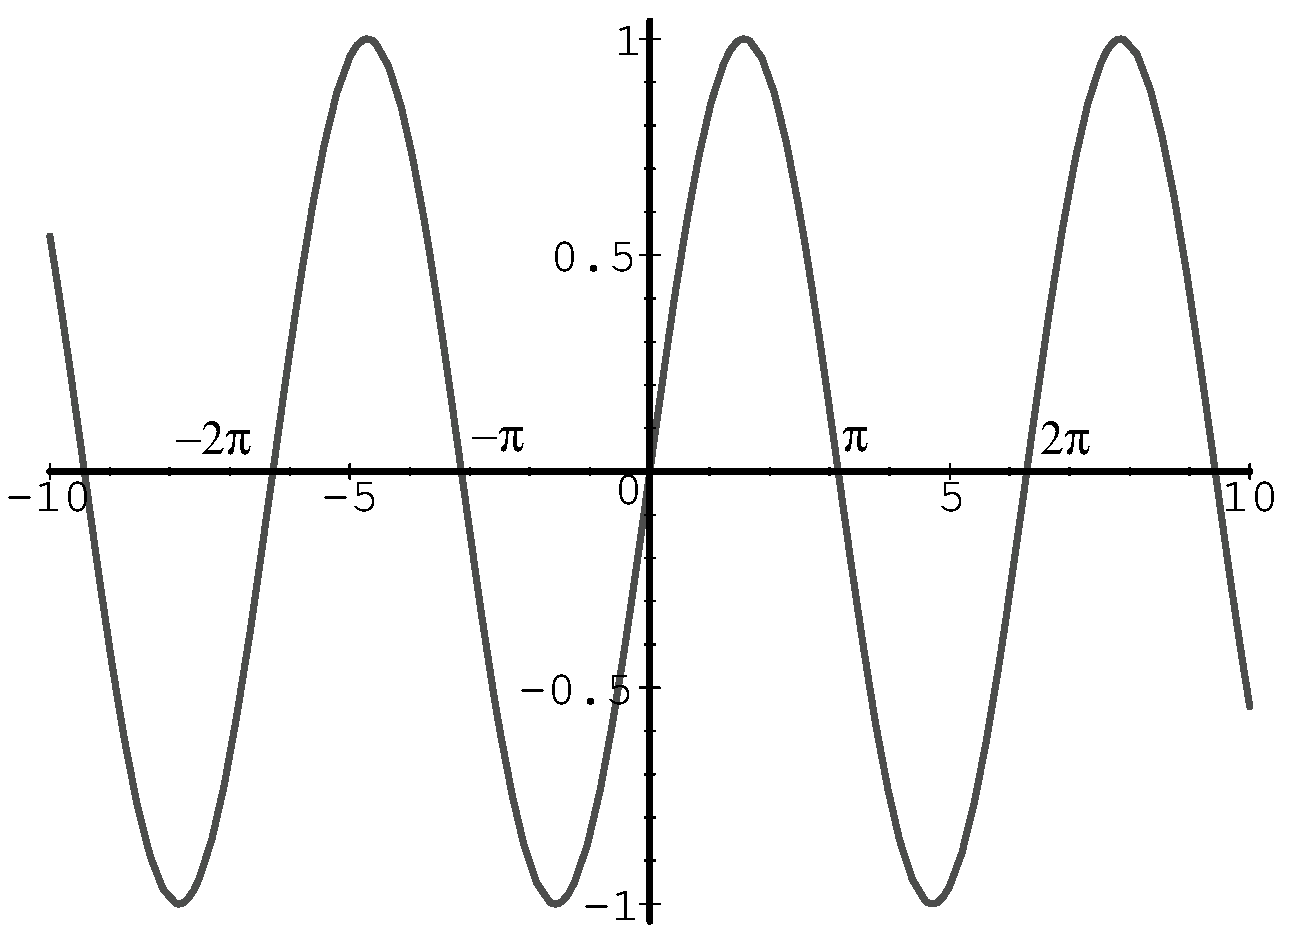
\includegraphics[width=0.75\hsize]
     {test.eps}
\caption{Sinusoid}
\end{figure}
\end{verbatim}
%
\end{comment}



%Some terms to find, define, and keep coherent:
%- Developer
%- The developer who uses models is called... (e.g. software architect modeler? doesn't mean anything)
%- The developer who uses code is called... (e.g. programmer)
%- Our method is for... called... (e.g. method for model code synchronization, method for architect/programmer collaboration, etc...)
%- Model is...
%- Code is...
%- Gap or difference ?
%- Background or practice or habits or profiles ? Maybe keep profile and choose one of the other?


\section{Introduction}
\label{sec:introduction}
The so-called Model-Driven Engineering (MDE) approach relies on two paradigms, abstraction and automation \cite{Mussbacher2014}. It is recognized as very efficient for dealing with complexity of today system. 
%Abstraction is the ability to provide simplified and focused view of a system and requires adequate modeling language. 
%Unified Modeling Language (UML) \cite{Specification2007} is nowadays the most used, educated, and documented modeling language. 
%Even, if a graphical language such as Unified Modeling Language (UML) \cite{Specification2007} is not the silver bullet for all software related concerns, it provides hence better support than text-based solutions for some concerns such as architecture and logical behavior of application development. 
Abstraction provides simplified and focused views of a system and requires adequate graphical modeling languages such as Unified Modeling Language (UML). Even, if the latter is not the silver bullet for all software related concerns, it provides better support than text-based solutions for some concerns such as architecture and logical behavior of application development. UML state machines (USMs) and their visual representations are much more suitable to describe logical behaviors of system entities than any equivalent text based descriptions. The gap from USMs to system implementation is reduced by the ability of automatically generating code from USMs  \cite{Booch1998, Douglass1999,Shalyto2006,Douglass1999}. 

Ideally, a full model-centric approach is preferred by MDE community due to its advantages \cite{Selic2012}. However, in industrial practice, there is significant reticence \cite{Hutchinson:2011:MEP:1985793.1985882} to adopt it.
On one hand, programmers prefer to
use the more familiar textual programming language. 
On the other hand, software architects, working at higher levels
of abstraction, tend to favor the use of models, and therefore
prefer graphical languages for describing the architecture of
the system.
%However, on the one hand, maintaining code generated from existing approaches is non-trivial. On the other hand our observation is that it is very difficult to come up with formalizations that yield such elegant code generation solutions \cite{6032552}. In other words, generated code must be manually modified to build fully operational applications. 
%On one hand there are traditional developers who prefer to implement the system by writing code, while on the other hand there are developers who prefer to use entirely models for the design and implementation of the system. 
The code modified by programmers and the model are then inconsistent. Round-trip engineering (RTE) \cite{Hettel2008} is proposed to synchronize different software artifacts, model and code in this case \cite{Sendall}. RTE enables actors (software architect and programmers) to freely move between different representations \cite{Sendall} and stay efficient with their favorite working environment. 

%After code modifications, round-trip engineering (RTE) is needed to make the model and code consistent, which is a critical aspect to meet quality and performance constraint required from project managers today. 
Unfortunately, current industrial tools such as for instance Enterprise Architect \cite{sparxsystems_enterprise_2014} and IBM Rhapsody\cite{ibm_rhapsody} only support structural concepts for RTE such as those available from class diagrams and code. Compared to RTE of class diagrams and code, RTE of USMs and code is non-trivial. It requires a semantical analysis of the source code, code pattern detection and mapping patterns into USM elements. 
This is a hard task, since mainstream programming languages such as C++ and JAVA do not have a trivial mapping between USM elements and source code statements.

For software development, one may wonder whether this RTE is doable. That is, why do the industrial tools not support the propagation of source code modifications back to original state machines? Several possible reasons to this lack are (1) the gap between USMs and code, (2) not every source code modification can be reverse engineered back to the original model, and (3) the penalty of using transformation patterns facilitating the reverse engineering that may not be the most efficient (e.g. a slightly larger memory overhead). 
%in the mind of these tools' vendors, users always make changes to models rather than to code. Generated code, in these tools, is therefore not supposed to be changed directly.  
 
%In this paper, we address the RTE of UML State Machine diagrams and its related generated code. We propose a RTE approach consisting of a forward process which generates code by using transformation patterns, and a backward process which is based on code pattern detection to update the original state machine model from the modified generated code. From the proposed approach, we implemented a prototype and conducted several experiments on different aspects of the round-trip engineering to verify the proposed approach. 



%Model-driven engineering (MDE) is a development methodology aiming to increase software productivity and quality by allowing different stakeholders to contribute to the system description \cite{Mussbacher2014}. MDE considers models as first-class artifacts and generates code from higher abstraction level models. Recent survey \cite{1030} has revealed that industries are gaining the adoption of code generation into software development life-cycle. Although many tools and research prototypes can generate executable code from models, generated code could be manually modified by programmers, e.g. skeleton code generated from UML \cite{Specification2007} class diagrams. Models and the generated code are therefore out of synchronization. Round-trip engineering \cite{Aßmann200333, Hettel2008, E-ESE-120044648} (RTE) is proposed to keep the artifacts synchronized.

%RTE supports synchronizing different software artifacts, model and code in this case, and thus enabling actors (software architect and programmers) to freely move between different representations \cite{Sendall}. Tools such as for instance Enterprise Architect \cite{sparxsystems_enterprise_2014}, Visual Paradigm \cite{visual}, and AndroMDA \cite{_andromda_} provide RTE but most of them are only applicable for system structure models such as class diagrams.  

%This study addresses the RTE of UML State Machine (SM) and object-oriented programming languages such as C++ and JAVA. SM is widely used in practice for modeling the behavior of complex systems, notably reactive, real-time embedded systems. There are several approaches to generating source code from state machines or state charts such as nested switch/if statements \cite{Booch1998}, state-event-table \cite{Douglass1999, Duby2001}, and state pattern \cite{Allegrini2002,Shalyto2006,Douglass1999}. Unfortunately, the generated code from these approaches is very difficult for programmers to maintain without an appropriate supporting tool. RTE is impossible in these approaches even with very small changes such as changing transition targets or actions made to code. The reason behind this impossibility is that, in mainstream programming languages such as C++, JAVA, (1) there are not equivalents between SMs and source code statements and (2) the code generation pattern of these approaches has not been chosen with RTE in mind.

%This paper addresses the RTE of UML state-machines and object-oriented programming languages such as C++ and JAVA. The forward  engineering of the approach takes as input a state-machine and executes two transformations. The first is UML to UML by utilizing several transformation patterns such as the double-dispatch approach presented in \cite{spinke_object-oriented_2013} and the second is a generation of code from the transformed UML. Traceability information is stored, during the transformations. In the backward direction, a verification is executed by the code pattern detection to verify the correctness of the code before the backward process taking as input the modified generated code, the UML classes, the original state-machine and mapping information together merges changes from code to the state-machine. We implemented a prototype supporting RTE of state-machine and C++ code, and conducted several experiments on different aspects of the RTE to verify the proposed approach. To the best of our knowledge, our implementation is the first tool supporting RTE of SM and code. 
%The prototype also improves the collaboration between MDE developers and traditional programmers in developing reactive complex embedded systems.

This paper addresses the RTE of USMs and object-oriented programming languages such as C++ and JAVA. The main idea is to utilize transformation patterns from USMs to source code that aggregates code segments associated with a USM element into source code methods/classes rather than scatters these segments in different places. Therefore, the reverse direction of the RTE can easily statically analyze the generated code by using code pattern detection and maps the code segments back to USM elements. Specifically, in the forward direction, we extend the double dispatch pattern presented in \cite{spinke_object-oriented_2013}. Traceability information is stored during the transformations. We implemented a prototype supporting RTE of state-machine and C++ code, and conducted several experiments on different aspects of the RTE to verify the proposed approach. To the best of our knowledge, our implementation is the first tool supporting RTE of SM and code. 

To sum up, our contribution is as followings:
\begin{itemize}
  \item An approach to round-tripping USMs and object-oriented code.
  \item A first tooling prototype supporting RTE of USMs and C++ code.
  \item An evaluation of the proposed approach including:
  \begin{itemize}
 	 \item An automatic evaluation of the proposed RTE approach with the prototype.% including 300 random generated SM models containing 80 states, more than 230 transitions, more than 250 actions and around 180 events for each.
  	 %\item A complexity analysis of the approach and performance evaluation.
  	 \item A comparison and collaboration of two software development practices including working at the model level and at the code level.
  	 \item A lightweight evaluation of the semantic conformance of the runtime execution of generated code.
  	\end{itemize}
\end{itemize}

The remaining of this paper is organized as follows: Our proposed approach is detailed in Section \ref{sec:approach}. The implementation of the prototype is described in Section \ref{sec:implementation}. Section \ref{sec:experiments} reports our results of experimenting with the implementation and our approach. Section \ref{sec:related_works} shows related work. The conclusion and future work are presented in Section \ref{sec:conclusion}.


\section{Approach}
\noindent
\tb{State}

%%%%
\section{Conclusion}


%\section*{Appendix}
%Appendixes, if needed, appear before the acknowledgment.

\section*{Acknowledgment}
This work is motivated by....


\balance
\bibliographystyle{IEEEtran}
%\bibliography{refs}



\end{document}
